\chapter[Storyboard]{Storyboard}

\section{Storyboard no Papel}

\subsubsection{Contexto}

\textbf{Pessoas envolvidas:} 
	Pessoas comuns

\textbf{Ambiente}
	Dentro de casa

\textbf{Tarefas}
	Procurar restaurante

\textbf{Os passos envolvidos}
	Procura categoria restaurante
	Procura pelo tipo de restaurante
	Visualiza a localização do restaurante

\textbf{Quais tarefas estão ilustradas}
Visualizar a localização do restaurante

\textbf{Qual a motivação de usar a aplicação}
	O storyboard apresentado nessa secção apresenta um contexto no qual um casal decide buscar um restaurante através da categoria gastronomia do site Curta Mais.

\subsection{Storyboard na Ferramenta}

\begin{figure}[H]
	\begin{center}
		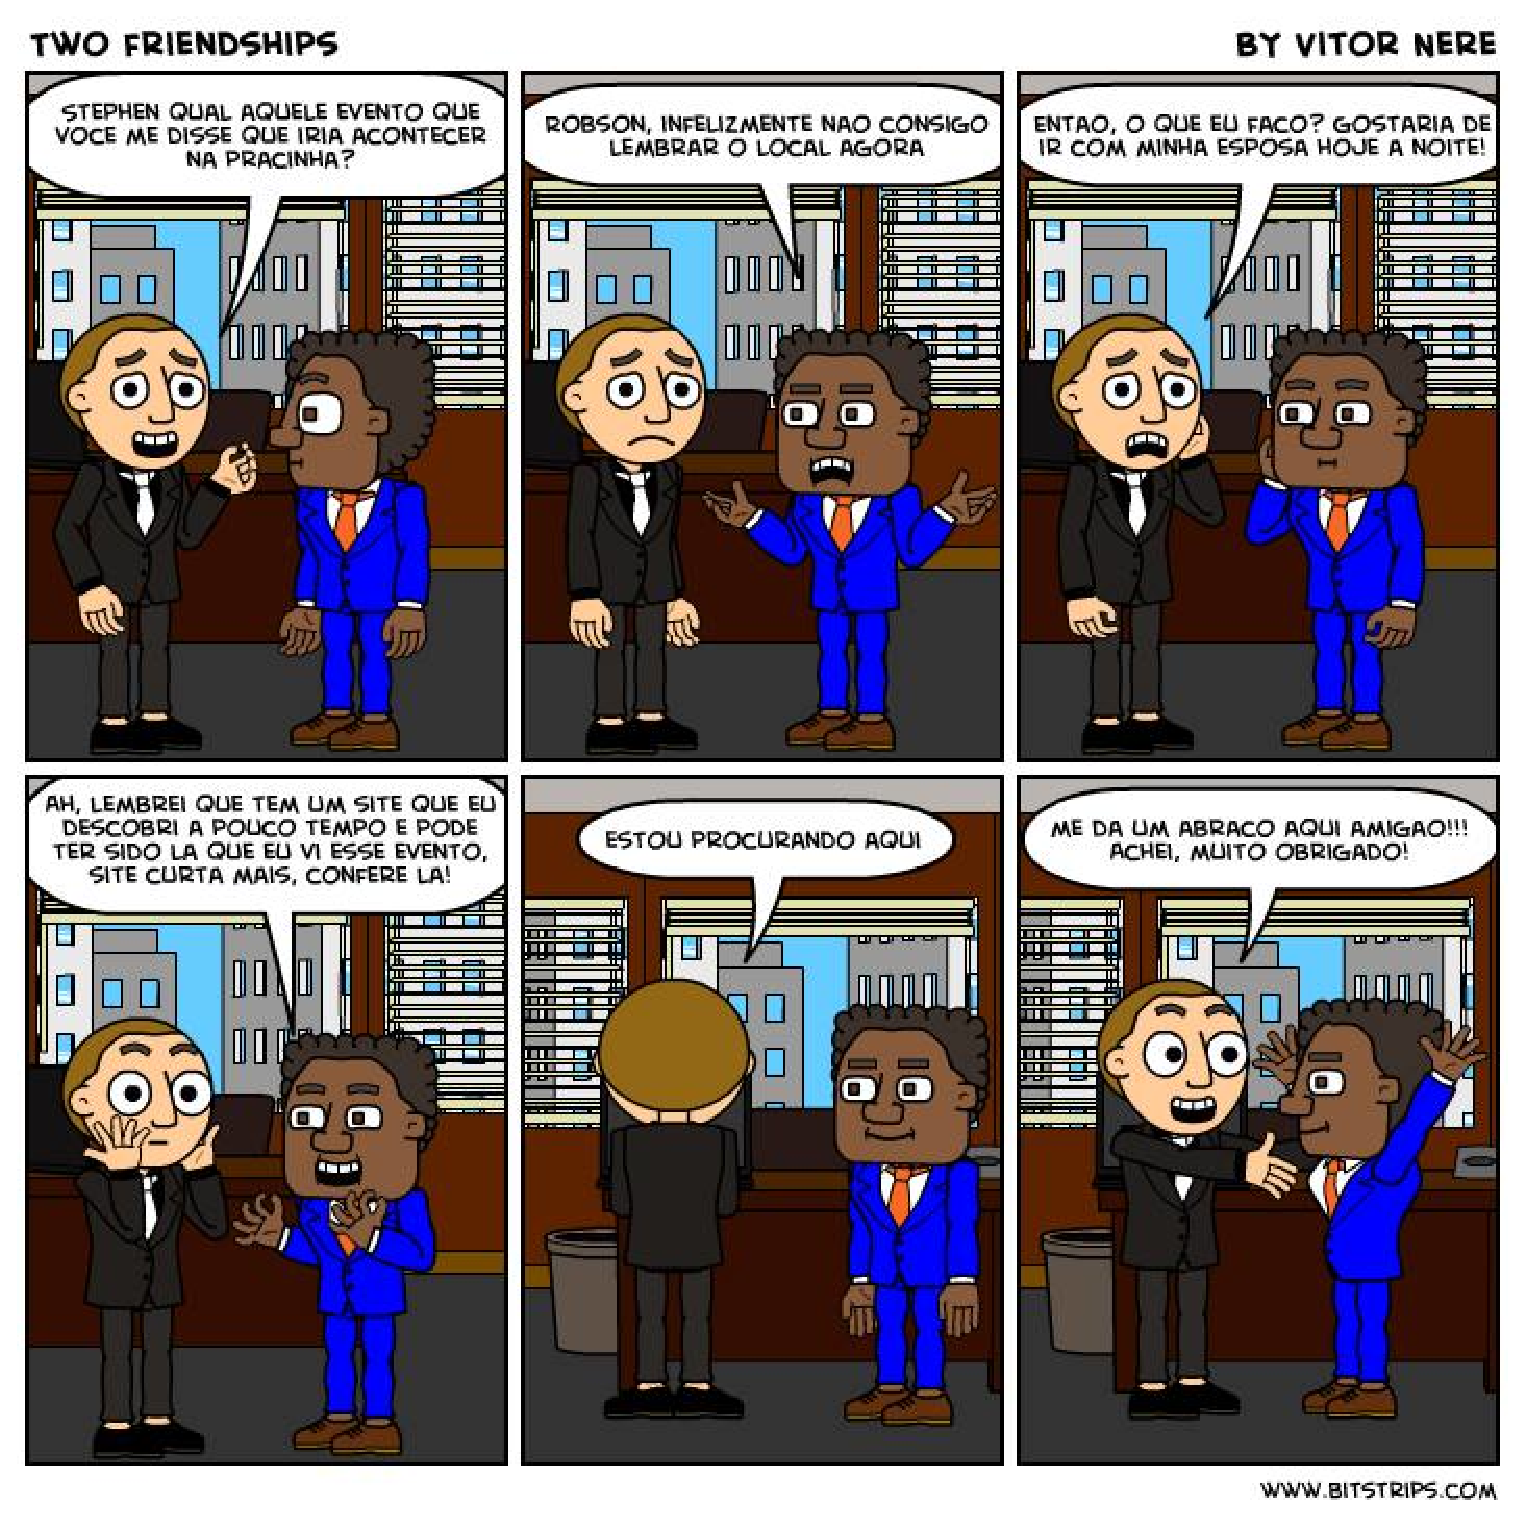
\includegraphics[keepaspectratio,scale=0.6]{figuras/bitstrip.eps}
		\caption{Storyboard - Two Friends}
	\end{center}
\end{figure}

\subsubsection{Contexto}

\textbf{Pessoas envolvidas:} 
	Pessoas comuns

\textbf{Ambiente}
	Dentro de casa

\textbf{Tarefas}
	Procurar site
	Procurar evento

\textbf{Os passos envolvidos}
	Procura pela categoria eventos
	Selecionar evento
	Visualiza o evento selecionado

\textbf{Quais tarefas estão ilustradas}
	Procurar pela opção todos eventos
	Visualizar que é o evento requerido e o local do evento

\textbf{Qual a motivação de usar a aplicação}
	O storyboard apresentado nessa secção apresenta um contexto em que um colega chega para outro querendo saber de um evento que ele tenha comentado anteriormente mas o colega não lembrava mais a respeito do evento e enquanto ele comentava o pq queria ir no evento, o colega lembrou que tem um site que informa sobre eventos gastronômicos e possivelmente foi por lá que ele ficou sabendo sobre o evento.